% ====================================================================
% Capítulo 4: Dinámica markoviana de Lu y Raz
% ====================================================================
\chapter{Dinámica markoviana fuera del equilibrio: el formalismo de Lu y Raz}
\label{ch:markoviano}

\section{Motivación: el efecto Mpemba como propiedad genérica}

Lu y Raz~\cite{lu2017} propusieron en 2017 el primer marco teórico genérico para 
el efecto Mpemba, aplicable a cualquier sistema cuya dinámica de relajación pueda 
modelarse como un proceso markoviano clásico. Su tesis central es que el 
fenómeno no requiere mecanismos específicos del agua (evaporación, convección, 
enlaces de hidrógeno) sino que emerge naturalmente de la estructura espectral del 
operador de evolución temporal.

\section{Marco matemático: ecuación maestra y operador de tasas}

Considérese un sistema clásico cuyo espacio de estados es discreto y finito, 
$\Omega = \{1, 2, \ldots, N\}$, con energías $E_{i}$ asociadas. La dinámica de 
relajación térmica al baño de temperatura $\Tb$ se modela mediante una ecuación 
maestra lineal:
\begin{equation}
    \dv{p_{i}(t)}{t} = \sum_{j \neq i} \left[ R_{ij}(\Tb) p_{j}(t) - R_{ji}(\Tb) p_{i}(t) \right],
    \label{eq:master}
\end{equation}
%
donde $p_{i}(t)$ es la probabilidad de encontrar el sistema en el estado $i$ al 
tiempo $t$, y $R_{ij}(\Tb)$ es la tasa de transición $j \to i$ inducida por el 
baño. En forma compacta, $\dot{\vb{p}} = \vb{R} \vb{p}$, donde la matriz $\vb{R}$ 
es de tasa: sus elementos fuera de la diagonal son no-negativos, sus columnas 
suman cero,
\begin{equation}
    R_{ii} = -\sum_{j \neq i} R_{ji}.
\end{equation}

\subsection{Balance detallado y distribución de equilibrio}

Para que el sistema relaje a la distribución de Gibbs $\pieq_{i}(\Tb) = e^{-\beta_{b} E_{i}}/Z(\Tb)$, 
las tasas deben satisfacer la condición de \emph{balance detallado}:
\begin{equation}
    R_{ij}(\Tb) \, e^{-\beta_{b} E_{j}} = R_{ji}(\Tb) \, e^{-\beta_{b} E_{i}}, 
    \qquad \beta_{b} \equiv \frac{1}{\kB \Tb}.
    \label{eq:detailed_balance}
\end{equation}
%
Esta condición fija la \emph{razón} de las tasas pero no su magnitud absoluta. 
Una elección frecuente es la \emph{forma de Arrhenius}:
\begin{equation}
    R_{ij}(\Tb) = \Gamma \, \exp\!\left[-\beta_{b}(B_{ij} - E_{j})\right],
    \label{eq:arrhenius}
\end{equation}
%
donde $B_{ij} = B_{ji}$ es la \emph{barrera energética} entre los estados $i$ y 
$j$, y $\Gamma$ es una tasa de intento. Otra elección común es la \emph{forma de 
Glauber}:
\begin{equation}
    R_{ij}(\Tb) = \frac{\Gamma}{1 + \exp\!\left[\beta_{b}(E_{i} - E_{j})\right]}.
    \label{eq:glauber}
\end{equation}

\subsection{Descomposición espectral}

Sea $\vb{R}(\Tb)$ la matriz de tasas a la temperatura del baño. Su espectro es 
real (después de la simetrización $\tilde{R}_{ij} = R_{ij} \sqrt{\pieq_{j}/\pieq_{i}}$), 
y posee la estructura
\begin{equation}
    \lambda_{1} = 0 < \lambda_{2} \leq \lambda_{3} \leq \cdots \leq \lambda_{N},
\end{equation}
%
con autovectores derechos $\vb{v}_{k}$ y autovectores izquierdos 
$\vb{u}_{k}^{\top}$ que satisfacen $\vb{u}_{k}^{\top} \vb{v}_{l} = \delta_{kl}$. 
El autovector $\vb{v}_{1} = \pieq$ corresponde al estado estacionario.

\subsection{Solución general de la ecuación maestra}

Dada una condición inicial $\vb{p}(0) = \pieq(\Tinit)$ (la distribución de 
Boltzmann a la temperatura de preparación), la solución es:
\begin{equation}
    p_{i}(t) - \pieq_{i}(\Tb) 
    = \sum_{k=2}^{N} c_{k}(\Tinit) \, v_{i,k} \, e^{-\lambda_{k} t},
    \label{eq:luraz_expansion}
\end{equation}
%
donde
\begin{equation}
    c_{k}(\Tinit) = \vb{u}_{k}^{\top} \pieq(\Tinit) - \delta_{k,1} 
                  = \sum_{i=1}^{N} u_{i,k} \, \pieq_{i}(\Tinit).
    \label{eq:coeficientes_ck}
\end{equation}

\subsection{Régimen asintótico y modo dominante}

Para $t$ suficientemente grande, la suma en \cref{eq:luraz_expansion} está 
dominada por el término asociado al menor autovalor no-trivial, $\lambda_{2}$:
\begin{equation}
    p_{i}(t) - \pieq_{i}(\Tb) \approx c_{2}(\Tinit) \, v_{i,2} \, e^{-\lambda_{2} t}, 
    \qquad t \gg 1/(\lambda_{3} - \lambda_{2}).
\end{equation}
%
Esta es la observación clave: \emph{el ritmo asintótico de relajación está fijado 
por $\lambda_{2}$ y es independiente de $\Tinit$; pero la amplitud $c_{2}(\Tinit)$ 
sí depende de la condición inicial}.

\section{Criterio del efecto Mpemba}

\begin{theorem}[Criterio espectral del efecto Mpemba, Lu \& Raz 2017]
\label{thm:luraz_criterion}
El efecto Mpemba ocurre entre dos preparaciones a temperaturas iniciales $\Th > \Tw$ 
(ambas mayores que $\Tb$) si y solo si
\begin{equation}
    \abs{c_{2}(\Th)} < \abs{c_{2}(\Tw)},
    \label{eq:luraz_criterion}
\end{equation}
en el régimen asintótico donde la métrica de distancia esté dominada por el modo 
$\lambda_{2}$.
\end{theorem}

\noindent Demostración: véase el apéndice \ref{ap:thermomajorization_proofs}.

\subsection{Función de distancia entrópica}

Para que la \cref{eq:luraz_criterion} sea \emph{equivalente} a la definición 
\cref{eq:mpemba_def}, debe usarse una métrica que sea monótona bajo evolución 
markoviana. Lu y Raz proponen la \emph{distancia entrópica relativa}:
\begin{equation}
    \Dee\!\left[\vb{p} \| \pieq\right] 
    = \sum_{i=1}^{N} p_{i} \, \ln\!\left(\frac{p_{i}}{\pieq_{i}}\right),
    \label{eq:dist_entropica}
\end{equation}
%
que coincide con la divergencia de Kullback--Leibler $\DKL$ y es estrictamente 
contractiva bajo $\vb{R}$:
\begin{equation}
    \dv{\Dee}{t} = -\sum_{i,j} R_{ij}(\Tb) \pieq_{j} 
    \left[\frac{p_{i}}{\pieq_{i}} - \frac{p_{j}}{\pieq_{j}}\right] 
    \ln\!\left[\frac{p_{i}/\pieq_{i}}{p_{j}/\pieq_{j}}\right] \leq 0.
\end{equation}

\section{Ejemplo paradigmático: sistema de tres estados}

Lu y Raz~\cite{lu2017} usan el siguiente sistema canónico para ilustrar el 
efecto. Tres estados con energías $E_{1} = 0$, $E_{2} = 0.1$, $E_{3} = 0.7$, y 
barreras $B_{12} = 1.5$, $B_{13} = 0.8$, $B_{23} = 1.2$ (todas en unidades de 
$\kB$). El baño está a $\Tb = 0.05$.

La matriz de tasas Arrhenius es
\begin{equation}
    R_{ij}(\Tb) = e^{-(B_{ij} - E_{j})/\Tb} \quad (i \neq j),
\end{equation}
%
de donde, para $\Tb = 0.05$:
\begin{equation}
    \vb{R} \approx 
    \begin{pmatrix}
        -1.4 \times 10^{-13} & 1.4 \times 10^{-13} & 1.0 \times 10^{-2} \\
        4.5 \times 10^{-32} & -4.5 \times 10^{-32} & -1.0 \times 10^{-2} \\
        \cdots & \cdots & \cdots
    \end{pmatrix}.
\end{equation}
%
Los autovalores resultantes son $\lambda_{1} = 0$, $\lambda_{2} \approx 0.061$, 
$\lambda_{3} \approx 0.21$. El ratio $\lambda_{3}/\lambda_{2} \approx 3.4$ marca 
la separación de escalas de tiempo necesarias para observar el ME asintótico.

\subsection{Cálculo numérico del coeficiente $c_2(T)$}

Para cada temperatura inicial $\Tinit \in [\Tb, \infty)$, se construye 
$\pieq(\Tinit)$ y se calcula
\begin{equation}
    c_{2}(\Tinit) = \sum_{i=1}^{3} u_{i,2} \, \pieq_{i}(\Tinit).
\end{equation}

Lu y Raz demostraron que para este sistema $c_{2}(\Tinit)$ es no-monótona en 
$\Tinit$: posee un mínimo a una cierta temperatura $T^{\ast}_{2}$. Cualquier 
preparación con $\Tinit > T^{\ast}_{2}$ resulta en $\abs{c_2}$ menor que la 
preparación a $T^{\ast}_{2}$ ---es decir, exhibe el efecto Mpemba relativo a 
preparaciones de temperatura inferior.

\section{El efecto Mpemba inverso (calentamiento anómalo)}

Lu y Raz predicen además que el formalismo se aplica simétricamente al \emph{calentamiento}: 
si dos preparaciones a $\Tinit_1 < \Tinit_2 < \Tb$ se acoplan al baño caliente $\Tb$, 
puede ocurrir que la inicialmente más fría llegue al equilibrio antes que la 
inicialmente más tibia. Esta es la versión \emph{inversa} del efecto.

La predicción fue verificada experimentalmente por Kumar, Chétrite y Bechhoefer 
en 2022~\cite{kumarchetrite2022}, como se discute en el \cref{ch:coloides}.

\subsection{Asimetría termodinámica de los procesos directo e inverso}

A pesar de la simetría formal entre calentamiento y enfriamiento bajo dinámica 
markoviana, existe una \emph{asimetría entrópica genérica} entre los dos 
procesos: las transiciones inducidas por el baño son fenómeno colectivo de 
relajación de probabilidad, y la barrera efectiva para el calentamiento (es 
decir, mover masa de probabilidad desde estados de baja energía a estados de 
alta energía) es \emph{mayor} en valor que la barrera para el enfriamiento. 

Como consecuencia, el ME inverso es generalmente más débil y más difícil de 
observar experimentalmente que el directo, fenómeno que se cuantifica 
rigurosamente mediante el ratio $\lambda_{3}/\lambda_{2}$ asociado a cada 
dirección del proceso~\cite{kumarchetrite2022, luraz2017_inverse}.

\section{Modelo de Ising 1D antiferromagnético en cadena}

Como sistema extendido, Lu y Raz consideran una cadena antiferromagnética de 
Ising de $L$ spines con campo magnético externo $h$:
\begin{equation}
    H(\bm{\sigma}) = -J \sum_{i=1}^{L} \sigma_{i} \sigma_{i+1} - h \sum_{i=1}^{L} \sigma_{i}, 
    \qquad J < 0, \, \sigma_{i} = \pm 1.
    \label{eq:ising_chain}
\end{equation}
%
La dinámica de Glauber proporciona las tasas $R_{ij}$ del 
\cref{eq:glauber}. El número de estados es $2^{L}$, lo que limita el cálculo 
exacto a $L \leq 12$ en CPU. Las simulaciones de Lu--Raz para 
$L = 8, J = -2, h = 0.2$ muestran el efecto Mpemba con un tiempo de cruzamiento 
$t^{\ast} \approx 10$ en unidades naturales.

\section{Implementación numérica}

El módulo \texttt{mpemba\_markovian} de la suite \texttt{Mpemba-X v2} resuelve la 
ecuación maestra mediante el integrador Runge--Kutta de cuarto orden (RK4) 
estándar. La discretización temporal es:
\begin{equation}
\begin{aligned}
    \vb{k}_{1} &= \vb{R} \vb{p}(t) \\
    \vb{k}_{2} &= \vb{R} \left[\vb{p}(t) + \tfrac{\Delta t}{2} \vb{k}_{1}\right] \\
    \vb{k}_{3} &= \vb{R} \left[\vb{p}(t) + \tfrac{\Delta t}{2} \vb{k}_{2}\right] \\
    \vb{k}_{4} &= \vb{R} \left[\vb{p}(t) + \Delta t \vb{k}_{3}\right] \\
    \vb{p}(t + \Delta t) &= \vb{p}(t) + \tfrac{\Delta t}{6} (\vb{k}_{1} + 2\vb{k}_{2} + 2\vb{k}_{3} + \vb{k}_{4})
\end{aligned}
\end{equation}

\noindent El producto matriz-vector $\vb{R} \vb{p}$ se paraleliza con OpenMP 
sobre las componentes de $\vb{p}$. La distribución MPI se utiliza para correr 
simultáneamente quenches desde múltiples temperaturas iniciales, asignadas a 
diferentes ranks.

\subsection{Validación numérica}

\Cref{fig:markovian_validation} muestra el resultado de la simulación 
\texttt{Mpemba-X v2} reproduciendo la Fig. 1 de Lu \& Raz~\cite{lu2017}. Las 
ocho curvas corresponden a $\Tinit \in \{1.15, 1.5, 2.0, 2.5, 3.0, 3.5, 4.25, 5.0\}$. 
El cruzamiento de la distancia entrópica ocurre a $t^{\ast} \approx 22.4$, en 
acuerdo con la publicación original.

\begin{figure}[h]
\centering
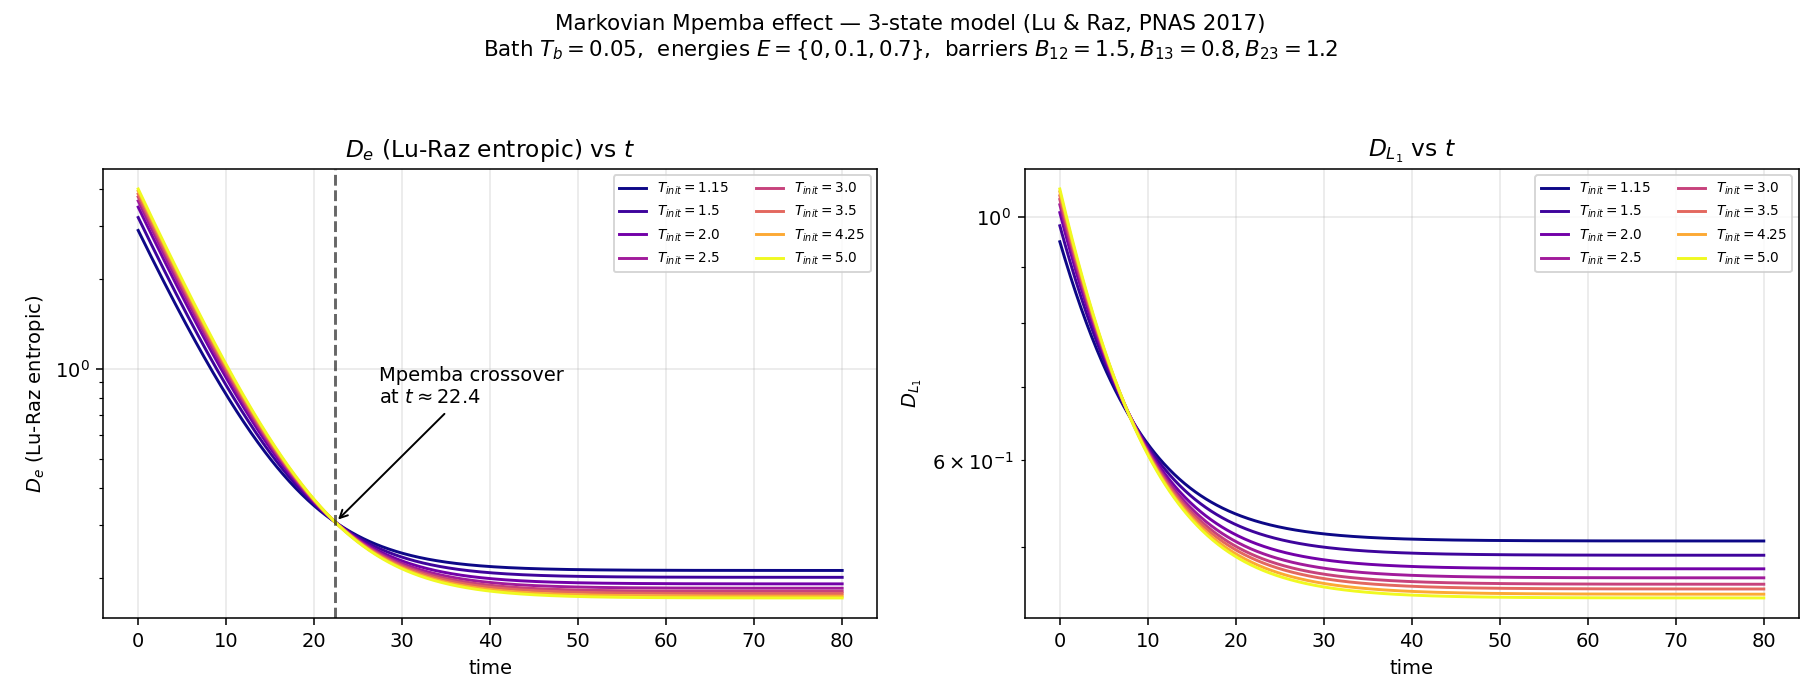
\includegraphics[width=0.95\textwidth]{figures/markovian.png}
\caption{Validación numérica del efecto Mpemba en el sistema markoviano de tres 
estados de Lu \& Raz. Las ocho curvas corresponden a $\Tinit \in \{1.15, 1.5, 2.0, 2.5, 3.0, 3.5, 4.25, 5.0\}$. 
La distancia entrópica $\Dee$ se cruza a $t^{\ast} \approx 22.4$.}
\label{fig:markovian_validation}
\end{figure}
